% Created 2015-09-25 Fri 22:27
\documentclass[11pt]{article}
\usepackage[utf8]{inputenc}
\usepackage[T1]{fontenc}
\usepackage{fixltx2e}
\usepackage{graphicx}
\usepackage{longtable}
\usepackage{float}
\usepackage{wrapfig}
\usepackage{rotating}
\usepackage[normalem]{ulem}
\usepackage{amsmath}
\usepackage{textcomp}
\usepackage{marvosym}
\usepackage{wasysym}
\usepackage{amssymb}
\usepackage{capt-of}
\usepackage[hidelinks]{hyperref}
\tolerance=1000
\usepackage[utf8]{inputenc}
\usepackage{commath}
\usepackage{pgf}
\usepackage{tikz}
\usetikzlibrary{shapes,backgrounds}
\usepackage{marginnote}
\usepackage{listings}
\usepackage{enumerate}
\usepackage{algpseudocode}
\usepackage{algorithm}
\usepackage{mathtools}
\usepackage{pldoc}
\usetikzlibrary{arrows,automata}
\setlength{\parskip}{16pt plus 2pt minus 2pt}
\renewcommand{\arraystretch}{1.6}
\DeclareMathOperator{\Neg}{Neg}
\author{Oleg Sivokon}
\date{\textit{<2015-09-07 Mon>}}
\title{Assignment 12, Authomata Theory}
\hypersetup{
 pdfauthor={Oleg Sivokon},
 pdftitle={Assignment 12, Authomata Theory},
 pdfkeywords={Automata Theory, Formal Languages, Assignment},
 pdfsubject={Second assignment in the course 20440 Automata and Formal Languages},
 pdfcreator={Emacs 25.0.50.1 (Org mode 8.3beta)}, 
 pdflang={English}}
\begin{document}

\maketitle
\tableofcontents

\definecolor{codebg}{rgb}{0.96,0.99,0.8}
\definecolor{codestr}{rgb}{0.46,0.09,0.2}
\lstset{%
  backgroundcolor=\color{codebg},
  basicstyle=\ttfamily\scriptsize,
  breakatwhitespace=false,
  breaklines=false,
  captionpos=b,
  framexleftmargin=10pt,
  xleftmargin=10pt,
  framerule=0pt,
  frame=tb,
  keepspaces=true,
  keywordstyle=\color{blue},
  showspaces=false,
  showstringspaces=false,
  showtabs=false,
  stringstyle=\color{codestr},
  tabsize=2
}
\lstnewenvironment{maxima}{%
  \lstset{%
    backgroundcolor=\color{codebg},
    escapeinside={(*@}{@*)},
    aboveskip=20pt,
    captionpos=b,
    label=,
    caption=,
    showstringspaces=false,
    frame=single,
    framerule=0pt,
    basicstyle=\ttfamily\scriptsize,
    columns=fixed}}{}
}
\makeatletter
\newcommand{\verbatimfont}[1]{\renewcommand{\verbatim@font}{\ttfamily#1}}
\makeatother
\verbatimfont{\small}%
\clearpage

\section{Problems}
\label{sec:orgheadline19}

\subsection{Problem 1}
\label{sec:orgheadline4}
\begin{enumerate}
\item Build an NFA for the language over alphabet \(\{a,b\}\) where words must
start with \(bab\) and end in \(b\).
\item Build an NFA for the language over alphabet \(\{a,b,c\}\), defined as
follows: \(L = \{w \;|\; \exists n,m,k \in \mathbb{N}.(w = a^nb^mc^k \land
      \abs{w} \mod 2 = 0)\}\).
\item Build an NFA for the language over alphabet \(\{a,b\}\), s.t. it contains
all words with substring \(aba\) repeated at least twice.
\end{enumerate}

\subsubsection{Answer 1}
\label{sec:orgheadline1}
\begin{tikzpicture}[->,>=stealth',shorten >=1pt,auto,node distance=2.8cm,
                    semithick]

  \node[initial,state]   (A)              {$q_0$};
  \node[state]           (B) [right of=A] {$q_1$};
  \node[state]           (C) [right of=B] {$q_2$};
  \node[accepting,state] (D) [right of=C] {$q_3$};
  \node[state]           (E) [below of=D] {$q_4$};

  \path (A) edge              node {b} (B)
        (B) edge              node {a} (C)
        (C) edge              node {b} (D)
        (D) edge              node {a} (E)
            edge [loop above] node {b} (D)
        (E) edge              node {b} (D)
            edge [loop right] node {a} (E);
\end{tikzpicture}

\emph{The nodes where automaton dies are not shown.}

The language accepted by this automaton must start with the prefix \(bab\) as
can be seen in diagram above.  The only accepting state has transitions
pointing at it only on inputs \(b\), thus all words accepted by this language
must end in \(b\).

Conversely, if the words start with the prefix \(bab\), then we must reach the
statate \(\hat{\delta}(bab, q_0) = q_4\).  From \(q_4\) the input can be either
accepted, since it already ends in any number of \(b\), or it may follow
through to \(q_4\) and whenever \(b\) is encountered in the input---return to
\(q_3\).  Since all execution path will thus lead to the accepting state on
\(b\) or to rejecting state on \(a\), I conclude that all words with prefix \(bab\)
and ending in \(b\) are accepted by the described automaton.

\subsubsection{Answer 2}
\label{sec:orgheadline2}
A regular expression to summarize the effort: \((((aa)^*((bb)^*(cc)^*) +
    (b(bb)^*c(cc)^*))) + (a(aa)^*((b(bb)^*(cc)^*) + (b(bb)^*(cc)^*)))\).

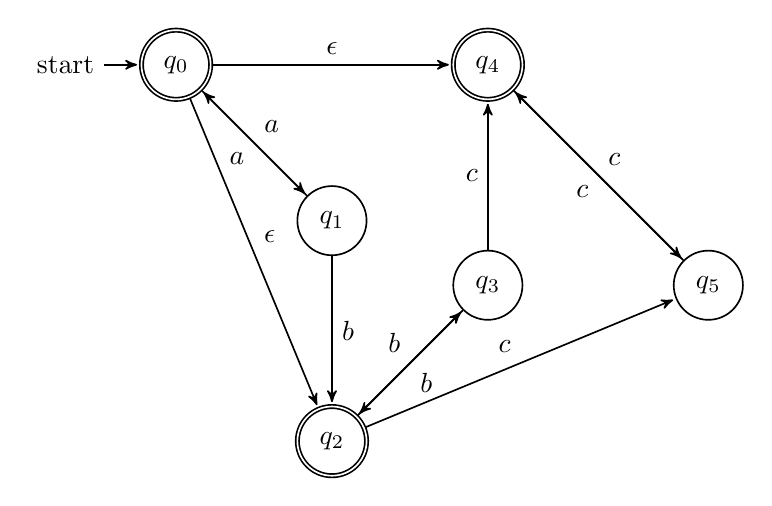
\begin{tikzpicture}[->,>=stealth',shorten >=1pt,auto,node distance=2.8cm,
                    semithick]

  \node[accepting,initial,state]   (A)              {$q_0$};
  \node[state]                     (B) [below right of=A] {$q_1$};
  \node[accepting,state]           (C) [below of=B] {$q_2$};
  \node[state]                     (D) [above right of=C] {$q_3$};
  \node[accepting,state]           (E) [above of=D] {$q_4$};
  \node[state]                     (F) [right of=D] {$q_5$};

  \path (A) edge node {$a$}        (B)
            edge node {$\epsilon$} (C)
            edge node {$\epsilon$} (E)
        (B) edge node {$a$}        (A)
            edge node {$b$}        (C)
        (C) edge node {$b$}        (D)
            edge node {$c$}        (F)
        (D) edge node {$b$}        (C)
            edge node {$c$}        (E)
        (E) edge node {$c$}        (F)
        (F) edge node {$c$}        (E);
\end{tikzpicture}

Essentially, what happens in this diagram is as follows:
\begin{enumerate}
\item On first input we decide whether the prefix starts with \(a\), \(b\) or \(c\).
\item Once decided, we parse more of the prefix.
\begin{itemize}
\item If the prefix was \(c\), we make sure there is even number of \(c\).
\item If the prefix started with \(b\), we create two branches, one will pick
the non-accepting state of the bit of automaton processing \(c\) prefix
once we counted even number of \(b\) inputs, and an accepting state
otherwise.
\item If our prefix was \(a\), then we will proceed similarly to the previous
case, however, we will switch roles: on odd number of \(a's\), we will
switch to an accepting state and to a non-accepting state otherwise.
\end{itemize}
\end{enumerate}

\subsubsection{Answer 3}
\label{sec:orgheadline3}
The diagram below can be also given by the regular expression:
\(((ab)^*b^*)^*aba(ba + (((ab)^*b^*)aba))(a + b)^*\).  An easier, but a
sloppier way to write the same regexp would be:
\((a + b)^*(ababa + (aba(a + b)^*aba))(a + b)^*\).

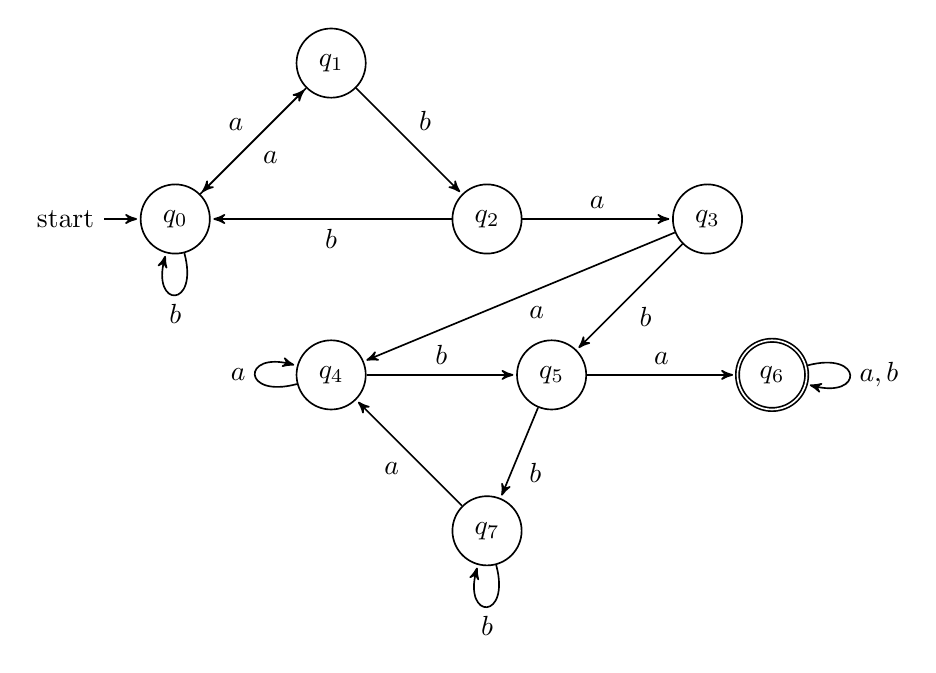
\begin{tikzpicture}[->,>=stealth',shorten >=1pt,auto,node distance=2.8cm,
                    semithick]

  \node[initial,state]   (A)                    {$q_0$};
  \node[state]           (B) [above right of=A] {$q_1$};
  \node[state]           (C) [below right of=B] {$q_2$};
  \node[state]           (D) [right of=C]       {$q_3$};
  \node[state]           (E) [below left of=C]  {$q_4$};
  \node[state]           (F) [below left of=D]  {$q_5$};
  \node[accepting,state] (G) [right of=F]       {$q_6$};
  \node[state]           (H) [below right of=E] {$q_7$};

  \path (A) edge [loop below] node {$b$}   (B)
            edge              node {$a$}   (B)
        (B) edge              node {$a$}   (A)
            edge              node {$b$}   (C)
        (C) edge              node {$a$}   (D)
            edge              node {$b$}   (A)
        (D) edge              node {$a$}   (E)
            edge              node {$b$}   (F)
        (E) edge [loop left]  node {$a$}   (E)
            edge              node {$b$}   (F)
        (F) edge              node {$a$}   (G)
            edge              node {$b$}   (H)
        (G) edge [loop right] node {$a,b$} (G)
        (H) edge              node {$a$}   (E)
            edge [loop below] node {$b$}   (E);
\end{tikzpicture}

Put in words: skip over repetitions of \(bb\) possibly preceded by \(a\), until
encountering \(aba\) substring.  Once that happens, consider the prefix of the
second \(aba\) substring found.  If the next input is \(b\), continue matching,
else---bail out and essentially repeat the previously described procedure.

\subsection{Problem 2}
\label{sec:orgheadline8}
Prove or disprove that pairs of regular expressions to follow accept the same
language.
\begin{enumerate}
\item \((0(10^*)^*)^*+1^*\) and \((1+0)^*\).
\item \((1+0)^+\) and \((0^*1)^*(1^*0)^++(0^*1)^+\).
\item \(1^*(0^*10^*)^*\) and \((101^*)^*1^*\).
\end{enumerate}

\subsubsection{Answer 3}
\label{sec:orgheadline5}
Two expressions are not equivalent.  \((1+0)^*\) matches any binary string,
while \((0(10^*)^*)^*+1^*\) doesn't match any binary string containing with a
prefix 00 or more consequtive zeros.

\subsubsection{Answer 4}
\label{sec:orgheadline6}
Two expressions are equivalent.  \((0^*1)^+\) will match any binary at least
one character long string edning in 1, while \((1^*0)^+\) will match any
binary string at least one character long ending in 0.  The union of these
two expressions will match all binary strings of length at least 1, which is
equivalent to \((1+0)^+\).  The \((0^*1)^*\) of the second expression plays no
role (is redundant).

\subsubsection{Answer 5}
\label{sec:orgheadline7}
Teo expressions are not equivalent.  \((101^*)^*1^*\) will not match string
containing 00 or more consequent zeros as a substring, while this is not a
problem for \(1^*(0^*10^*)^*\).

\subsection{Problem 3}
\label{sec:orgheadline10}
Write a regular expression for the language over alphabet \(\{a,b\}\) s.t. all
words in this language start with either \(aa\) or \(bbb\) and none of them
contains substring \(bab\).

\subsubsection{Answer 6}
\label{sec:orgheadline9}
The desired regex is \((bbb^+)^*(aa^+b^*)^*\).

\subsection{Problem 4}
\label{sec:orgheadline13}
Write an algorithm which accepts a regular expression \(r\) and produces a
language \(\overline{L[r]}\).

\subsubsection{Answer 7}
\label{sec:orgheadline12}
The basic idea is to convert given regular expression to NFA, from NFA to
DFA, switch roles of accepting and rejecting states, then convert the DFA
into a regular expression again.  I wrote concerte implementation for this
algorithm.  The documentation to my code is given in \ref{sec:orgheadline11}, the code
itself can be found together with this document (it is not included for
brevity).

\begin{description}
\item[{String to regexp}] This step requires writing a recursive parser (since
we need to balance parenthesis).  Given a string containing regular
expression this step produces an AST of regular expression code
(further AST).
\item[{Regexp to NFA}] This step starts off with creating a starting state and a
distinct accepting state.  It recursively processes every node of AST
and for each one of four node types it appends nodes to NFA:
\begin{description}
\item[{terminal}] No nodes are added, only an arc between two active nodes.
\item[{concatenation}] One node is added between two currently active nodes,
and each node is processed further with the added node as either its
source or its destination.
\item[{union}] No nodes are added.  This is similar to the \texttt{terminal} step,
except both regexp are expanded further.
\item[{star}] Add \(\epsilon\)-transition from both the source and the
destination nodes to the node currently processed.  Add
\(\epsilon\)-transition from the destination to the source.
\end{description}
\item[{NFA to DFA}] At first, arrange all transitions into a matrix \(M_{i,q}\)
indexed by inputs \(i\), including \(\epsilon\) and states \(q\).  Create a
new matrix \(M'_{j,p}\) indexed by inputs concatenated to \(\epsilon^*\)
and new states \(p\).  New states are obtained as follows: Select a cell
\(m = M_{i,q}\), \(m\) will be the set of all states reacheable on input
\(i\) from state \(q\), suppose \(m = \{q_n, q_{n+1}, \dots q_{n+m}\}\).
Now, for each \(p \in \{q_n, \dots q_{n+m}\}\) find the cell \(e =
         M_{\epsilon, p}\).  The union of these cells is the label of target DFA.
\item[{Flip rejecting and accepting states}] This step is trivial: make switch
the roles of all states.  Note that this requires the often omitted
``dead'' state.
\item[{DFA to regexp}] For each state \(S\) of the DFA record the union of all
states immediatel reacheable from the given state in a form of a
grammar rule \(S_a \to iS_b\).  Substitute rules into each other to
eliminate non-terminals as follows:
\begin{itemize}
\item \(S_n \to i\{\epsilon\} \implies S_n \to i\).
\item \(S_n \to iS_n \implies S_n \to i^*\).
\item \(S_n \to iS_m, S_m \to jS_k \implies S_n \to ijS_k\).

It is useful to apply set-theoretic identities, such as distributivity
of union over concatenation, eg. \(xz \cup yz = (x \cup y)z\) to produce
a better regular expression.
\end{itemize}
\item[{Serialize regexp to string}] Recursively visit every node of AST and
substitue the node contents with its string representation.
\end{description}


Example code inverts a regular expression \(x(y+x)^*+z\).  However, the
current version of this code lacks the ability to optimize the produced
regular expressions.

\lstset{language=prolog,label= ,caption= ,captionpos=b,numbers=none}
\begin{lstlisting}
:- use_module(automata).

replace_tex(Out) -->
    [], { Out = "" } ;
    "*", replace_tex(Y),
    { string_concat("^*", Y, Out) } ;
    [603], replace_tex(Y),
    { string_concat("\\epsilon", Y, Out) } ;
    [X], replace_tex(Y),
    { text_to_string([X], Xs), string_concat(Xs, Y, Out) }.

assignment_12a :-
    invert_regex(`x(y+x)*+z`, Regex),
    string_codes(Regex, Codes),
    phrase(replace_tex(X), Codes),
    format('$$~w$$', [X]).
\end{lstlisting}

\((((zz+(zy+(zx+(yz+(yy+(yx+xz))))))+((\epsilon+y)+((zz+(zy+(zx+(yz+(yy+(yx+xz))))))((z+(y+x)))^*+((xy+xx)z+(xy+xx)((y+x))^*))))+((xy+xx)zz+((xy+xx)zy+(xy+xx)zx))(\epsilon+((z+(y+x)))^*))\)
\((((zz+(zy+(zx+(yz+(yy+(yx+xz))))))+((\epsilon+y)+((zz+(zy+(zx+(yz+(yy+(yx+xz))))))((z+(y+x)))^*+((xy+xx)z+(xy+xx)((y+x))^*))))+((xy+xx)zz+((xy+xx)zy+(xy+xx)zx))(\epsilon+((z+(y+x)))^*))\)


\subsection{Problem 5}
\label{sec:orgheadline15}
Build a DFA from given NFA:

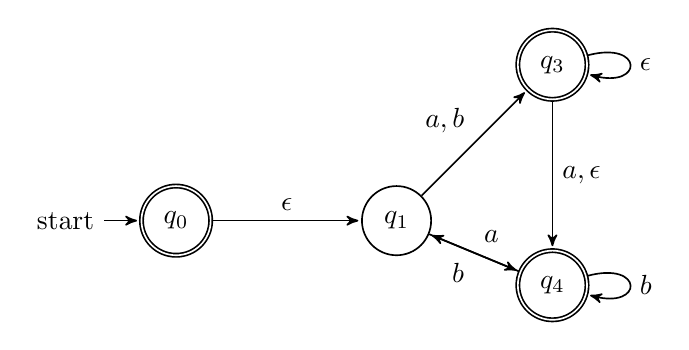
\begin{tikzpicture}[->,>=stealth',shorten >=1pt,auto,node distance=2.8cm,
                    semithick]

  \node[accepting,initial,state]   (A)                    {$q_0$};
  \node[state]                     (B) [right of=A]       {$q_1$};
  \node[accepting,state]           (C) [above right of=B] {$q_3$};
  \node[accepting,state]           (D) [below of=C]       {$q_4$};

  \path (A) edge              node {$\epsilon$}   (B)
        (B) edge              node {$a,b$}        (C)
            edge              node {$a$}          (D)
        (C) edge [loop right] node {$\epsilon$}   (D)
            edge              node {$a,\epsilon$} (D)
        (D) edge              node {$b$}          (B)
            edge [loop right] node {$b$}          (D);
\end{tikzpicture}

\subsubsection{Answer 8}
\label{sec:orgheadline14}
The corresponding DFA can be written as:

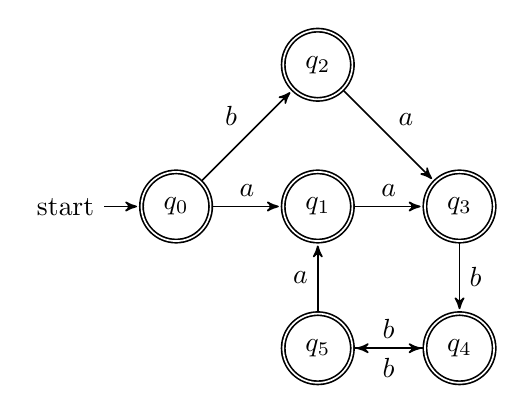
\begin{tikzpicture}[->,>=stealth',shorten >=1pt,auto,node distance=1.8cm,
                    semithick]

  \node[accepting,initial,state]   (A)              {$q_0$};
  \node[accepting,state]           (B) [right of=A] {$q_1$};
  \node[accepting,state]           (C) [above of=B] {$q_2$};
  \node[accepting,state]           (D) [right of=B] {$q_3$};
  \node[accepting,state]           (E) [below of=D] {$q_4$};
  \node[accepting,state]           (F) [left of=E]  {$q_5$};

  \path (A) edge  node {$a$}   (B)
            edge  node {$b$}   (C)
        (B) edge  node {$a$}   (D)
        (C) edge  node {$a$}   (D)
        (D) edge  node {$b$}   (E)
        (E) edge  node {$b$}   (F)
        (F) edge  node {$b$}   (E)
            edge  node {$a$}   (B);
\end{tikzpicture}

\emph{Nodes where automata dies are not shown.}

\subsection{Problem 6}
\label{sec:orgheadline17}
Write a regular expression for the diagram below:

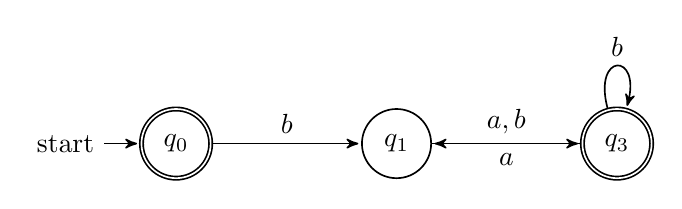
\begin{tikzpicture}[->,>=stealth',shorten >=1pt,auto,node distance=2.8cm,
                    semithick]

  \node[accepting,initial,state]   (A)              {$q_0$};
  \node[state]                     (B) [right of=A] {$q_1$};
  \node[accepting,state]           (C) [right of=B] {$q_3$};

  \path (A) edge              node {$b$}   (B)
        (B) edge              node {$a,b$} (C)
        (C) edge [loop above] node {$b$}   (D)
            edge              node {$a$}   (B);
\end{tikzpicture}

\emph{Nodes where the automata dies are not shown.}

\subsubsection{Answer 9}
\label{sec:orgheadline16}
The regular expression for the diagram above: \(\epsilon + b((a + b)b^*)^+\).

\subsection{Problem 7}
\label{sec:orgheadline18}
Given regular expression \(r\) and \(L\), a language over \(\Sigma\) which
designates regular expression \(r\Sigma^*\).  Prove that unless \(L = \Sigma^*\)
and \(L = \emptyset\), there doesn't exist a regular expression \(s\) s.t.
\(s\Sigma^*\) designates \(\overline{L}\).
\section{Appendix A}
\label{sec:orgheadline11}
\bgroup
% This LaTeX document was generated using the LaTeX backend of PlDoc,
% The SWI-Prolog documentation system



\subsection{automata.pl: High-level predicates for dealing with regular expressions}

\label{sec:automata}

\begin{tags}
    \tag{See also}
\url{https://github.com/wvxvw/intro-to-automata-theory}
\end{tags}

This module defines predicates for searching and replacing in strings
using regular expressions.\vspace{0.7cm}

\begin{description}
    \predicate[det]{match_regex}{2}{+Regex, +String}
Evaluates to true if \arg{String} is accepted by \arg{Regex}.

\begin{tags}
    \tag{See also}
\predref{match_suffix_regex}{3}, \predref{match_all_regex}{3}
\end{tags}

    \predicate[det]{match_suffix_regex}{3}{+Regex, +String, -Suffix}
Evaluates to true if \arg{Suffix} is the remaining part of the \arg{String}
not matched by \arg{Regex}.

\begin{tags}
    \tag{See also}
\predref{match_regex}{2}, \predref{match_all_regex}{3}
\end{tags}

    \predicate[nondet]{match_all_regex}{3}{+Regex, +String, -Match}
Instantiates \arg{Match} to all possible matches of \arg{Regex} in \arg{String}.

\begin{tags}
    \tag{See also}
\predref{match_regex}{2}, \predref{match_suffix_regex}{3}
\end{tags}

    \predicate[det]{invert_regex}{2}{+Straight, -Inverted}
\arg{Inverted} is a regular expression accepting the complement language
of the regular expression \arg{Straight}.
\end{description}

\subsection{automata(ast): Grammar constituents used when parsing regular expressions}

\label{sec:ast}

\begin{tags}
    \tag{See also}
\url{https://github.com/wvxvw/intro-to-automata-theory}
\end{tags}

This module defines predicates for generating abstract syntax trees
representing regular expressions.\vspace{0.7cm}

\begin{description}
    \predicate[nondet]{rterminal}{1}{?Regex}
Evaluates to true if \arg{Regex} is either an atom or an empty list.
Empty list denotes empty string, atoms stand for characters of
the strings.

\begin{tags}
    \tag{See also}
\predref{runion}{2}, \predref{rstar}{1}, \predref{rconcat}{2}, \predref{regex}{1}
\end{tags}

    \predicate[det]{runion}{2}{+Regex1, +Regex2}
Evaluates to true if \arg{Regex1} and \arg{Regex2} are valid regular expressions
as defined in \predref{regex}{1}.

\begin{tags}
    \tag{See also}
\predref{runion}{2}, \predref{rstar}{1}, \predref{rconcat}{2}, \predref{regex}{1}
\end{tags}

    \predicate[det]{rstar}{1}{+Regex}
Evaluates to true if \arg{Regex} is a valid regular expressions
as defined in \predref{regex}{1}.

\begin{tags}
    \tag{See also}
\predref{rterminal}{1}, \predref{rstar}{1}, \predref{rconcat}{2}, \predref{regex}{1}
\end{tags}

    \predicate[det]{rconcat}{2}{+Regex1, +Regex2}
Evaluates to true if \arg{Regex1} and \arg{Regex2} are valid regular expressions
as defined in \predref{regex}{1}.

\begin{tags}
    \tag{See also}
\predref{runion}{2}, \predref{rterminal}{1}, \predref{rconcat}{2}, \predref{regex}{1}
\end{tags}

    \predicate[det]{regex}{1}{+Regex}
Evaluates to true if \arg{Regex} is either a \predref{runion}{2}, or a \predref{rstar}{1}, or
a \predref{rconcat}{2} or a \predref{rterminal}{1}.

\begin{tags}
    \tag{See also}
\predref{runion}{2}, \predref{rstar}{1}, \predref{rconcat}{2}, \predref{rterminal}{1}
\end{tags}
\end{description}

\subsection{automata(convert): Convert between different automata represenations}

\label{sec:convert}

\begin{tags}
    \tag{See also}
\url{https://github.com/wvxvw/intro-to-automata-theory}
\end{tags}

This module defines defines conversions between regular expression
AST, DFA represented as a list of transitions or as a table, and NFA
represented similarly to DFA.

This module also defines data types:

\begin{itemize}
    \item Transition record

\begin{code}
trn(from:integer, to:integer, input:input, acc:boolean)
\end{code}

To describe a single transition between states on some input.
\const{acc} is \const{true} whenever the target state is an accepting one.
    \item State record

\begin{code}
state(label, acc:boolean)
\end{code}

To describe states.
    \item Transition table row record

\begin{code}
row(state:state, trns:trns)
\end{code}

To describe all inputs for a given state.
    \item Transition table record

\begin{code}
table(inputs:list(input), tab:list(row))
\end{code}

To describe a complete table of transitions between all states
of some automata.
\end{itemize}

\vspace{0.7cm}

\begin{description}
    \predicate[det]{has}{3}{+Accessor, ?Value, ?Record}
Flips arguments for Accessr (the predicate generated to access
fields of the record).

    \predicate[det]{regex_to_nfa}{2}{+Regex, -Nfa}
Evaluates to true when given regular expression \arg{Regex} can be
decomposed into a list of transitions \arg{Nfa}.

\begin{tags}
    \tag{See also}
\predref{gexps}{3}
\end{tags}

    \predicate[det]{nfa_inputs}{2}{+Nfa, -Inputs}
Evaluates to true when \arg{Inputs} is the alphabet of the \arg{Nfa} automata.

    \predicate[det]{nfa_states}{2}{+Nfa, -States}
Evaluates to true when \arg{States} is the states of the \arg{Nfa} automata.

    \predicate[det]{reacheable_states}{4}{+Input, +Transitions, +Table, -States}
Evaluates to true when \arg{States} can be reached from all \arg{Transitions}
on given \arg{Input}. This also accounts for epsilon transitions.

    \predicate[det]{nfa_table}{2}{+Transitions, -Table:table}
Evaluates to true when \arg{Table} is the transitions table containing
all transitions given by \arg{Transitions}.

    \predicate[det]{nfa_to_dfa}{2}{+Nfa, -Dfa}
Evaluates to true when \arg{Dfa} accepts the same language as \arg{Nfa}.

    \predicate[det]{table_to_diagram}{2}{+Table, -Diagram}
Evaluates to true when \arg{Diagram} contains all the transitions
described in \arg{Table}.

    \predicate[det]{dfa_to_regex}{2}{+Dfa, -Regex}
Evaluates to true when \arg{Regex} accepts the same language as the
given \arg{Dfa}. \arg{Dfa} could be either a transitions table or a list of
all transitions.

    \predicate[det]{dfa_minimize}{2}{+Dfa, -Minimized}
Evaluates to true when \arg{Minimized} is the minimal DFA of \arg{Dfa}.
\end{description}

\subsection{automata(parser): DCG rules for parsing regular expressions}

\label{sec:parser}

\begin{tags}
    \tag{See also}
\url{https://github.com/wvxvw/intro-to-automata-theory}
\end{tags}

This module defines DCG rules for parsing regular expressions from
string.\vspace{0.7cm}

\begin{description}
    \predicate[det]{gstar}{3}{+Exp, +Prefix, -Suffix}
Parses a regular expression followed by an asterisk (the Kleene
operator). Instantiates its first term to the rstar AST nonterminal.

\begin{tags}
    \tag{See also}
\predref{rstar}{1}
\end{tags}

    \predicate[det]{gunion}{3}{+Exp, +Prefix, -Suffix}
Parses a union of two regular expressions joined by the \verb$+$ sign.
Instantiates its first term to the runion AST nonterminal.

\begin{tags}
    \tag{See also}
\predref{runion}{2}
\end{tags}

    \predicate[det]{gchar}{3}{+Exp, +Prefix, -Suffix}
Parses a single terminal character and instantiates it to
AST rterminal term.

\begin{tags}
    \tag{See also}
\predref{rterminal}{1}
\end{tags}

    \predicate[det]{gexps}{3}{+Tree, +Prefix, -Suffix}
Parses regular expression from the string \arg{Prefix} and instantiates
the \arg{Tree} to the parse \predref{regex}{1} term.

\begin{tags}
    \tag{See also}
\predref{regex}{1}
\end{tags}
\end{description}

\subsection{automata(printing): Predicates for pretty printing}

\label{sec:printing}

\begin{tags}
    \tag{See also}
\url{https://github.com/wvxvw/intro-to-automata-theory}
\end{tags}

This module defines predicates useful to print structures generated by
other automata modules.\vspace{0.7cm}

\begin{description}
    \predicate[det]{regex_to_string}{2}{+Exp, -Result}
Evaluates to true when given regular expression \arg{Exp} can be written
as \arg{Result} string.

\begin{tags}
    \tag{See also}
\predref{regex}{1}
\end{tags}

    \predicate[det]{format_table}{1}{+Table:table}
Pretty-prints the contents of the transitions table.

\begin{tags}
    \tag{See also}
\predref{nfa_to_dfa}{2}, \predref{nfa_table}{2}
\end{tags}
\end{description}

\subsection{automata(utils): Vairous utilitis for working with lists}

\label{sec:utils}

\begin{tags}
    \tag{See also}
\url{https://github.com/wvxvw/intro-to-automata-theory}
\end{tags}

This module defines several utilities for working with lists
used across multiple other automata modules.\vspace{0.7cm}

\begin{description}
    \predicate[det]{reflexive_pairs}{2}{+Source, -Pairs}
Evaluates to true when \arg{Pairs} contains lists of length 2 each of
which contains a unique pair from the elements of \arg{Source}. For
this purpose \verb$[X, Y]$ is the same as \verb$[Y, X]$.

    \predicate[det]{cmp_lists}{3}{+List1, +List2, -Op}
Lexicographically compares \arg{List1} and \arg{List2}. \arg{Op} is set to either
one of \verb$<$, \verb$=$ and \verb$>$ respectively.

    \predicate[det]{replace_all}{4}{+Searched, +Replacement, +Source, -Destination}
Evaluates to true when \arg{Destination} contains all the elements of
\arg{Source} with \arg{Searched} element replaced by \arg{Replacement}.

\begin{tags}
    \tag{See also}
\predref{replace_all_lift}{4}, \predref{replace_all_tree}{4}, \predref{replace_all_tree_lift}{4}
\end{tags}

    \predicate[det]{replace_all_lift}{4}{+Replacement, +Searched, +Source, -Destination}
Same as \predref{replace_all}{4} except that \arg{Replacement} element is
substituted for each of the elements of \arg{Searched} list.

\begin{tags}
    \tag{See also}
\predref{replace_all}{4}, \predref{replace_all_tree}{4}, \predref{replace_all_tree_lift}{4}
\end{tags}

    \predicate[det]{replace_all_tree}{4}{+Searched, +Replacement, +Source, -Destination}
Same as \predref{replace_all}{4} except that \arg{Searched} cannot be a list, and
all sublists of \arg{Source} are processed recursively.

\begin{tags}
    \tag{See also}
\predref{replace_all}{4}, \predref{replace_all_lift}{4}, \predref{replace_all_tree_lift}{4}
\end{tags}

    \predicate[det]{replace_all_tree_lift}{4}{+Searched, +Replacement, +Source, -Destination}
Same as \predref{replace_all_tree}{4} except that \arg{Replacement} element is
substituted for each of the elements of \arg{Searched} list.

\begin{tags}
    \tag{See also}
\predref{replace_all}{4}, \predref{replace_all_tree}{4}, \predref{replace_all_lift}{4}
\end{tags}
\end{description}


\egroup
\end{document}